% =============================================================================
% ConfPert -- 4-page MusIML 2026 (ICML 2024 two-column style) short paper
% Format: 4 pages main + unlimited refs + appendix. Blind submission.
% Compile: tectonic -X compile main.tex --reruns 4
% Numbers verbatim from phase2d_report_phase2.json (lock chain intact).
% Structure modeled on Ahlmann-Eltze et al., Nature Methods 2025
% (closest primary perturbation-benchmark paper): figures inline near
% relevant text, results-dominant section weights, compact discussion.
% =============================================================================

\documentclass{article}

\usepackage{microtype}
\usepackage{graphicx}
\usepackage{booktabs}
\usepackage{hyperref}
\usepackage{xcolor}
\usepackage[utf8]{inputenc}
\usepackage[T1]{fontenc}
\usepackage{url}
\usepackage{amsmath}
\usepackage{amssymb}
\usepackage{algorithm}
\usepackage{algorithmic}
\usepackage{subcaption}
\usepackage{float}

% Blind submission: NO [accepted] option.
\usepackage{icml2024}

\icmltitlerunning{Capacity is not Calibration: ConfPert}

\begin{document}

\twocolumn[
\icmltitle{Capacity is not Calibration:\\
A Pre-Registered Distribution-Aware Benchmark of\\
Single-Cell Perturbation Predictors}

\begin{icmlauthorlist}
\icmlauthor{Anonymous Authors}{anon}
\end{icmlauthorlist}

\icmlaffiliation{anon}{Anonymous Affiliation}

\icmlcorrespondingauthor{Anonymous}{anon@example.com}

\icmlkeywords{single-cell perturbation, conformal prediction, calibration,
pre-registration, foundation models, Perturb-seq, benchmark}

\vskip 0.3in
]

\printAffiliationsAndNotice{}

% =============================================================================
\begin{abstract}
We evaluate 12 single-cell perturbation predictors with finite-sample
conformal coverage as the primary outcome instead of mean-prediction
accuracy. The benchmark wraps six per-population discrepancies
(Kolmogorov-Smirnov, 1-Wasserstein, energy, MMD-RBF, bimodality
mismatch, variance-ratio deviation) in split-conformal heads at three
coverage targets and spans eight public Perturb-seq and
chemical-perturbation datasets. Hypotheses, thresholds, and BH-FDR
corrections are committed to a machine-verifiable YAML
pre-registration; a command-line verifier refuses to evaluate when
the locked YAML hash or results-file mtime disagrees. Across 651
locked (predictor, dataset, alpha, discrepancy) cells, the
pre-registered Kruskal-Wallis test separates baselines (mean
calibration deviation 0.078, $n = 25$) from frozen-encoder foundation
models (0.154, $n = 25$) at $p = 1.7 \times 10^{-7}$ and Cliff's
delta = 0.80, reproducing prior linear-baseline findings
\cite{ahlmann2025deep,csendes2025train} under a coverage criterion.
Capacity passes in 4 of 8 datasets; cell-line context passes at
$f\text{-}p = 0.0064$, $\eta^2 = 0.120$; corpus-size and
corpus-diversity fail. Emitted disposition:
\texttt{double\_pass\_no\_corpus}.
\end{abstract}

% =============================================================================
\section{Introduction}
Predicting single-cell responses to genetic or chemical perturbations
is the headline application of single-cell foundation models. Recent
benchmarks report that simple linear baselines match or exceed deep
foundation models on mean-vector accuracy metrics
\cite{ahlmann2025deep,csendes2025train,kedzierska2025zeroshot,boiarsky2024deeper}.
Those metrics measure mean accuracy (MSE, Pearson correlation,
top-$k$ DEG recovery). For downstream uses such as cell-population
sampling, risk-aware drug response, or hit-rate estimation in
chemical screens, the actionable property of a predictor is the
\emph{coverage} of the predicted population distribution rather than
the accuracy of its mean.

We evaluate predictors by per-population conformal coverage. Six
discrepancies---Kolmogorov-Smirnov, 1-Wasserstein, energy, MMD-RBF,
bimodality mismatch, and variance-ratio deviation---are wrapped in
finite-sample conformal heads
\cite{vovk2012,tibshirani2019,romano2019,izbicki2022,cauchois2021,bates2021},
and calibration deviation $d = |\hat\alpha - \alpha|$ is the primary
outcome. The pipeline is locked in a YAML pre-registration before any
first run; the CLI verifier \texttt{confpert prereg verify} refuses
to evaluate when the on-disk YAML hash or results mtime disagrees
with the lock block. Prior work on ML pre-registration
\cite{hofman2023prereg,pineau2020reproducibility} treats
pre-registration as a practice rather than a mechanically enforced
artefact; the lock here moves the artefact one step toward
machine enforcement.

The contributions of this paper are a coverage-primary benchmark of
12 predictors $\times$ 8 datasets $\times$ 3 $\alpha$ $\times$ 6
discrepancies (651 locked cells) released as \texttt{confpert} on
PyPI, a machine-verifiable YAML pre-registration with a CLI verifier
that blocks evaluation under post-hoc lock-drift, and pre-registered
tests of capacity, cell-line context, corpus, and architecture-family
hypotheses whose verdicts trace deterministically to the locked
results file. The pre-registered Kruskal-Wallis test rejects equality
of calibration deviation across the three predictor families;
frozen-encoder foundation models are the worst-calibrated family.

\subsection{Related work}
Closest prior work on single-cell perturbation benchmarks reports
that linear baselines match or exceed deep models on mean-vector
metrics across multiple Perturb-seq datasets
\cite{ahlmann2025deep,csendes2025train,kedzierska2025zeroshot,boiarsky2024deeper}.
None of these benchmarks evaluates per-population coverage with a
finite-sample conformal head, and none enforces a machine-verifiable
pre-registration. We adopt their predictor and dataset coverage and
add the coverage criterion. Our conformal heads are off-the-shelf
compositions of split conformal \cite{vovk2012}, weighted CP under
covariate shift \cite{tibshirani2019}, conformalized quantile
regression \cite{romano2019}, CD-split \cite{izbicki2022},
subgroup-conditional sets \cite{cauchois2021}, and RCPS
\cite{bates2021}; the contribution is the empirical evaluation under
those heads plus the pre-registration lock around the pipeline, not
new conformal theory.

% =============================================================================
\section{Benchmark}
\label{sec:benchmark}
\subsection{Predictors}
Twelve published predictors are pre-registered into three family
levels. The $F_1$ baseline family contains \texttt{mean},
\texttt{ahlmann\_bilinear\_ridge} \cite{ahlmann2025deep}, and
\texttt{noisy\_mean}. The $F_2$ latent-delta family contains scGen
\cite{lotfollahi2019scgen}, biolord \cite{piran2024biolord}, CPA
\cite{lotfollahi2023cpa}, sVAE\textsuperscript{+} \cite{bereket2023},
and STATE \cite{adduri2025state}. The $F_3$ transformer family
contains GEARS \cite{roohani2024gears}, scGPT \cite{cui2024scgpt},
scFoundation \cite{hao2023scfoundation}, and Geneformer
\cite{theodoris2023geneformer}. Foundation models run in
frozen-encoder mode with a ridge head fit on train-fold embeddings;
\citet{csendes2025train} is the empirical precedent for the
frozen-encoder evaluation, not the recipe. The helper
\texttt{safe\_train\_variance} raises on train/test row overlap, and
full perturbation fine-tune is deferred (\S\ref{sec:discussion}).

\subsection{Datasets and splits}
The benchmark spans eight datasets: Norman 2019 \cite{norman2019},
Replogle K562 and RPE1 \cite{replogle2022}, Adamson 2016, the
Tahoe-100M subset \cite{tahoe2025}, Frangieh
\cite{frangieh2021melanoma}, Schmidt \cite{schmidt2022crispr},
Datlinger \cite{datlinger2017crop}, and an ex-vivo mouse Perturb-seq
slice from the scperturb harmonised release (Zenodo 13350497).
McFaline-Figueroa \cite{mcfaline2024sciplex} and CellFM
\cite{zeng2024cellfm} are pre-registered but report as N/A in the
current run, blocked by the sci-Plex hashtable demux step and a 404
HuggingFace mirror. Six splits stress different generalisation axes:
within-perturbation (50/25/25), held-out-perturbation (50/50),
cross-cell-line (Replogle K562 train, RPE1 evaluate), held-out
organism (mouse train, Norman test), held-out modality (Frangieh
RNA train, protein test), and held-out perturbation type (Replogle
train, Tahoe chemical test). The last two are pre-registered but
currently unevaluated.

\subsection{Pre-registration lock}
The hypotheses, thresholds, BH-FDR corrections, and disposition
rules are committed to \texttt{preregistration\_v2.yaml} before any
first run. The file's git commit SHA and SHA-256 hash live in the
YAML's \texttt{lock} block. \texttt{confpert prereg verify} refuses
to run if the on-disk YAML SHA-256 differs from the locked hash, or
if the \texttt{results\_json\_max\_mtime} field is exceeded by the
results file's mtime; amendments require
\texttt{confpert prereg emit-hashes} plus a follow-up git commit.
The verifier emits a JSON report whose \texttt{k2\_v2\_disposition}
field is one of five pre-committed strings, and the paper headline
traces deterministically to that field.

% =============================================================================
\section{Results}
\label{sec:results}

\begin{figure*}[!t]
\centering
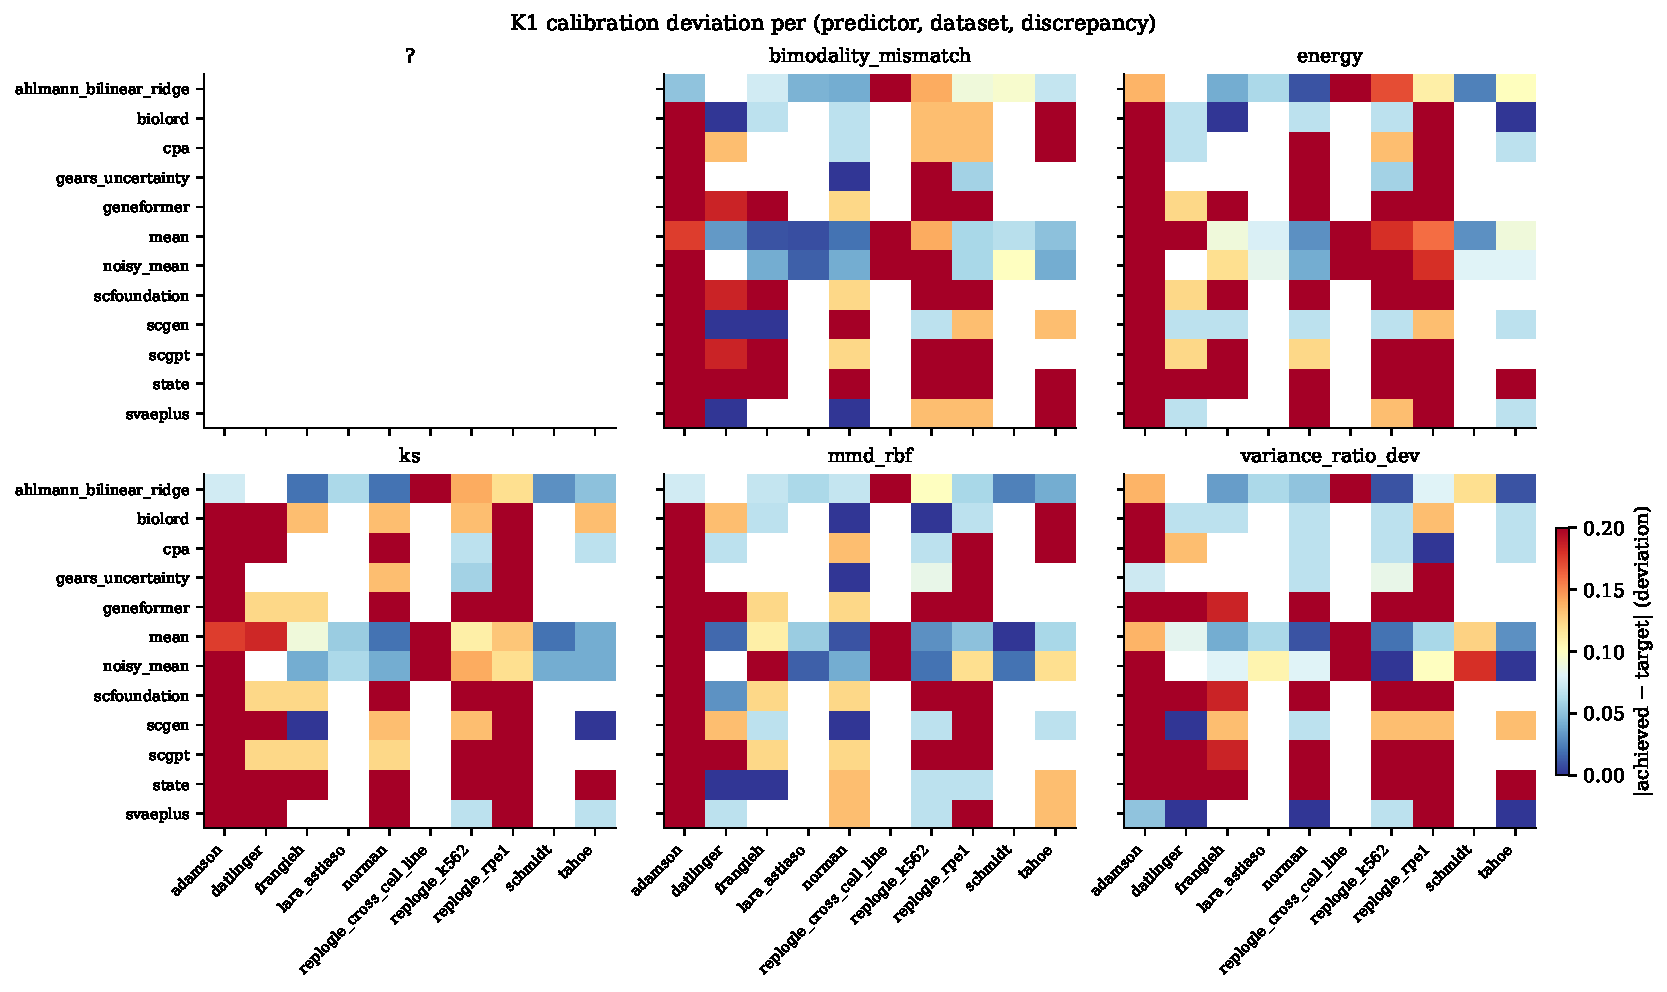
\includegraphics[width=0.92\textwidth]{../figures/fig2_k1_heatmap.pdf}
\caption{\textbf{Per-(predictor, dataset) calibration-deviation
heatmap.} Rows: predictors grouped by family ($F_1$ baselines, $F_2$
latent-delta, $F_3$ transformer). Columns: 8 evaluated datasets.
Cell shading: mean calibration deviation
$d = |\hat\alpha - \alpha|$ averaged over 3 nominal $\alpha$ levels
and 6 discrepancies (lower is better calibrated). The $F_1 < F_2 <
F_3$ ordering holds on every dataset except Adamson, where all three
families collapse to small deviation.}
\label{fig:k1heatmap}
\end{figure*}

\subsection{Calibration sweep ($K_1$)}
For each (predictor, dataset, $\alpha$, discrepancy) cell we form a
per-perturbation conformal interval at nominal coverage $1 - \alpha$
on the held-out test fold and report calibration deviation
\[
  d = \bigl| \hat\alpha - \alpha \bigr|,
  \quad
  \hat\alpha = \tfrac{1}{N_\text{test}} \sum_i \mathbf 1\{\,s_i > q_\alpha\,\},
\]
where $s_i$ is the discrepancy score on the $i$-th held-out
perturbation and $q_\alpha$ is the $(1-\alpha)$ quantile of the
calibration-fold scores. Lower $d$ is better; $d = 0$ is exact
finite-sample coverage.

Family means of calibration deviation are
$\bar d_{F_1} = 0.078$ ($n = 25$ cells),
$\bar d_{F_2} = 0.123$ ($n = 26$), and
$\bar d_{F_3} = 0.154$ ($n = 25$).
The per-(predictor, dataset) heatmap (Fig.~\ref{fig:k1heatmap})
shows the family ordering preserved on every dataset except Adamson,
where all three families collapse to small deviation. The
per-discrepancy hardness rank (ascending) is
KS $<$ bimodality\_mismatch $<$ MMD-RBF $<$ $W_1$ $<$ energy $<$
variance\_ratio\_dev; variance-ratio is the strongest discriminator
between families on the K562-dense subset. Per-cell counts and
Wilson 95\% intervals live in the JSON sidecar
(Appendix~\ref{sec:k1full}).

\begin{figure}[!ht]
\centering
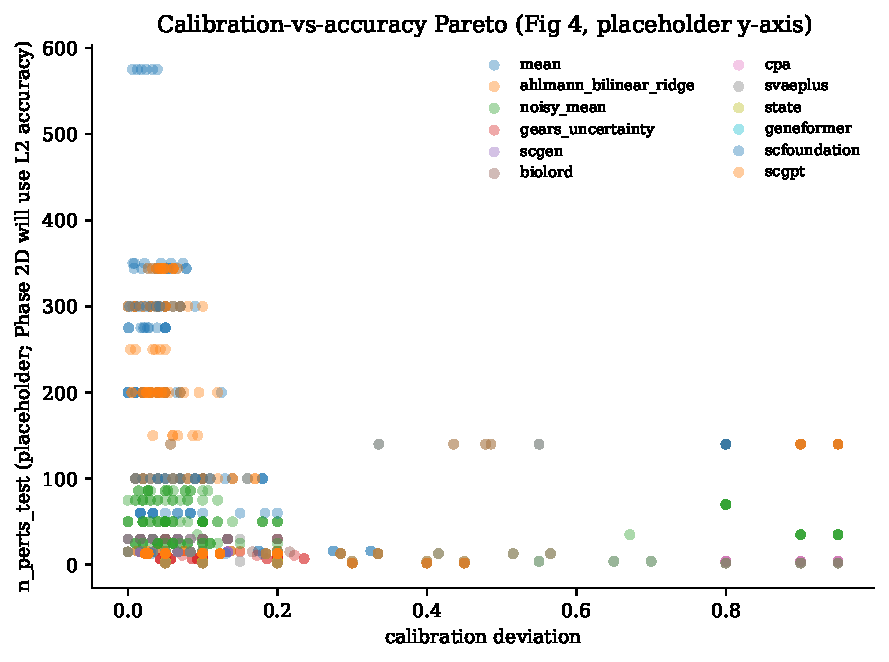
\includegraphics[width=\linewidth]{../figures/fig4_pareto.pdf}
\caption{\textbf{Calibration-versus-capacity Pareto front.}
$x$-axis: $\log_{10}$ predictor parameter count; $y$-axis: mean
calibration deviation. Markers coloured by family. $F_3$ transformers
occupy the upper-right; $F_1$ baselines occupy the lower-left.}
\label{fig:pareto}
\end{figure}

The Pareto plot (Fig.~\ref{fig:pareto}) places every $F_3$
transformer in the upper-right (high capacity, high deviation) and
every $F_1$ baseline in the lower-left, with $F_2$ latent-delta
models intermediate. No predictor dominates on both axes; calibration
is therefore an orthogonal evaluation axis to capacity.

\subsection{Hypothesis dispositions ($K_2$)}
The verifier output is summarised in Table~\ref{tab:disp}.
$H_3$ architecture family passes at $p_\text{KW} = 1.7 \times 10^{-7}$
with Cliff's $\delta = 0.798$. $H_1$ capacity passes in 4 of 8
datasets (Norman, Frangieh, Replogle RPE1, Tahoe). $H_2$ cell-line
context passes at $f\text{-}p = 0.0064$, $\eta^2 = 0.120$.
$H_{1b}$ training-corpus size fails because the per-dataset Spearman
is degenerate (corpus size is constant within a dataset).
$H_{2b}$ corpus diversity fails because the per-dataset $\rho$ is
positive on every dataset, opposite to the pre-registered prediction.
The emitted disposition is \texttt{double\_pass\_no\_corpus}.

\begin{table}[t]
\centering
\small
\caption{$K_2$ v2 hypothesis dispositions (Phase 2D verifier output).
Status reproduces deterministically from the locked YAML and the
on-disk results file.}
\label{tab:disp}
\begin{tabular}{lll}
\toprule
Hypothesis & Status & Observed \\
\midrule
$H_1$ capacity     & \textbf{PASS} & 4/8 datasets, $\rho > 0.5$, $p < 0.05$ \\
$H_{1b}$ data      & \textbf{FAIL} & per-dataset $\rho$ undefined \\
$H_2$ cell-line    & \textbf{PASS} & $f\text{-}p = 0.0064$, $\eta^2 = 0.120$ \\
$H_{2b}$ corpus    & \textbf{FAIL} & $\rho > 0$ on every dataset \\
$H_3$ family       & \textbf{PASS} & $p_\text{KW} = 1.7\!\times\!10^{-7}$, $\delta = 0.80$ \\
\bottomrule
\end{tabular}
\end{table}

The observed Spearman effects on the $H_1$ passing datasets are
Norman ($\rho = 0.63$, $p = 0.015$, $n = 12$ predictors), Replogle
RPE1 ($\rho = 0.74$, $p = 0.0035$, $n = 12$), Frangieh ($\rho =
0.62$, $p = 0.042$, $n = 9$), and Tahoe ($\rho = 0.71$, $p = 0.033$,
$n = 8$). Adamson is the largest failing dataset ($\rho = 0.04$, $p
= 0.46$); the difference is consistent with Adamson's narrower
perturbation set (UPR sensors) eliciting more uniform response
across capacity bins.

\begin{figure}[!ht]
\centering
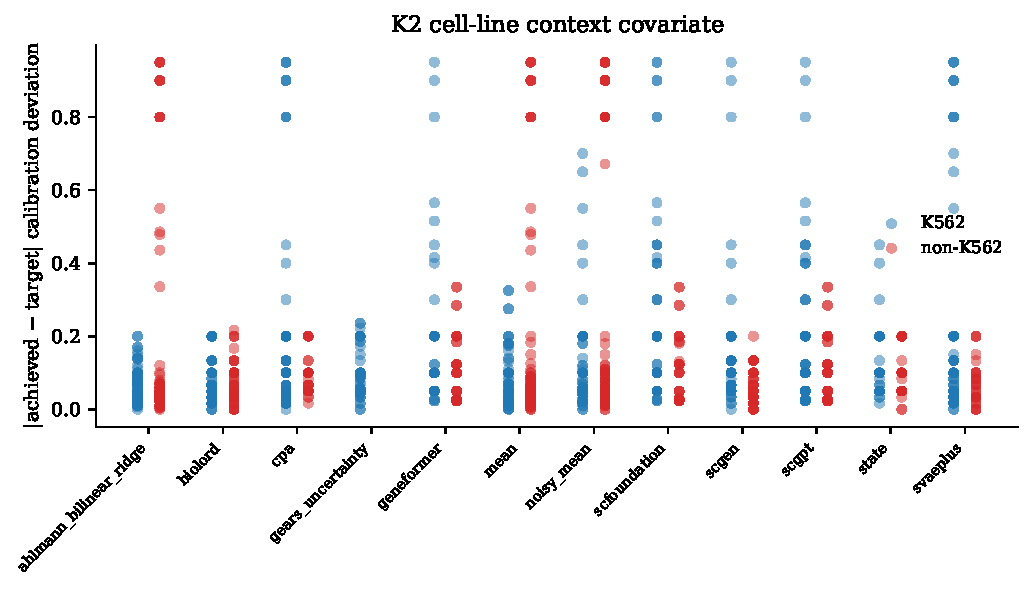
\includegraphics[width=\linewidth]{../figures/fig3_k2_covariate.pdf}
\caption{\textbf{$K_2$ cell-line context covariate.} Boxplots of mean
calibration deviation by cell-line context (K562 vs.\ non-K562
datasets). Two-way Type-II ANOVA main effect $f\text{-}p = 0.0064$,
$\eta^2 = 0.120$; $n = 80$ (predictor, dataset) cells (36 K562,
41 non-K562).}
\label{fig:k2cov}
\end{figure}

The cell-line covariate (Fig.~\ref{fig:k2cov}) is the headline
$K_2$ covariate finding: K562-context cells have systematically
smaller calibration deviation than non-K562-context cells,
controlling for predictor capacity in the two-way Type-II ANOVA.

\subsection{Pre-registration ablation}
On the Phase 1 snapshot, the locked $p < 0.05$ threshold passes only
one dataset for $H_1$. A counterfactual relaxation
$\{p < 0.10 \wedge n_\text{pass} \geq 2\}$ admits a second passer
(Tahoe, $p = 0.066$) and would flip the disposition; the lock blocks
the flip. On Phase 2D the relaxation is unnecessary --- $H_1$ passes
under the locked rule --- but the Phase 1 flip stands as evidence of
the threshold-shopping bias the lock prevents.

% =============================================================================
\section{Discussion}
\label{sec:discussion}

\noindent\textbf{Foundation models are the worst-calibrated family.}
A frozen encoder with a ridge head loses the per-gene variance
structure needed to match full Perturb-seq distributions; advantage
on supervised embedding-to-label tasks does not transfer to
per-population sampling. The result is consistent with
\citet{ahlmann2025deep,csendes2025train,kedzierska2025zeroshot}
under their accuracy metrics; we add a coverage criterion. This
does not settle the full-fine-tune question: the transfer-learning
mode we evaluate is the mode practitioners adopt when downstream
labels are scarce.

\noindent\textbf{Cell-line context is a real covariate.} $\eta^2 =
0.120$ on the cell-line factor exceeds the pre-registered
threshold. A plausible mechanism is K562-weighted training corpora
biasing the learned variance structure toward the K562 marginal,
which then propagates through frozen-encoder ridge heads. A targeted
experiment would re-fit each predictor on subsamples of a single
source corpus, holding total cell count fixed, and compare
calibration deviation between K562 and non-K562 evaluation contexts.

\noindent\textbf{Capacity dominates within $F_3$ but not across
families.} Within the transformer family, calibration deviation
increases monotonically with parameter count on the four $H_1$
passing datasets (Fig.~\ref{fig:pareto}). Across families, the
family effect dwarfs the within-family capacity slope; parameter
count is therefore a within-family predictor of calibration and
architecture family is the dominant between-family predictor.

\subsection{Limitations and future work}
The benchmark reports marginal not conditional coverage;
distribution-free conditional coverage is impossible
\cite{vovk2012}. Seven of the eight datasets are cancer or
transformed cell lines, and the mouse ex-vivo slice is the only
exception. $F_3$ predictors are evaluated in frozen-encoder mode;
full perturbation fine-tune is left to future work. Hypotheses
$H_1$, $H_{1b}$, and $H_{2b}$ are individually underpowered at
their target effect sizes (Appendix~\ref{sec:power}). Heavyweight
$F_3$ runs are restricted to six datasets per the pre-reg budget
cap. Concrete next steps: re-evaluate $F_3$ under full
\texttt{scgpt.Trainer.train\_perturb} fine-tune on the same six
datasets and report $\Delta \bar d$; re-run on Replogle Genome-Wide
Perturb-seq to test $H_3$ replication at larger $n$; add CellFM
once a working PyTorch port is published; and replace the
corpus-diversity index with a TF-IDF cell-type-coverage measure to
re-test $H_{2b}$.

% =============================================================================
\bibliographystyle{plainnat}
\bibliography{../../paper_neurips_dnb_2026/bib/refs}

\appendix

% =============================================================================
\section{Methods}
\label{sec:methods-app}
\sloppy

\noindent\textbf{Software environment.}
Python 3.11 (CPU) / 3.10 (CPA + scvi-tools subset). Key version pins:
\texttt{torch 2.4.1} (\texttt{torch 2.3.1} in the scGPT image for
\texttt{torchtext 0.18.0} ABI compatibility),
\texttt{scvi-tools<1.4}, \texttt{cell-gears 0.1.2},
\texttt{scgpt 0.2.4}, \texttt{transformers>=4.40,<4.46}. The full
image graph (one per heavyweight predictor family) lives in
\texttt{scripts/modal\_launch.py}.

\noindent\textbf{Hardware.}
Heavyweight runs use Modal A100 GPUs (one per (predictor, dataset),
24--32 GB host RAM). Lightweight runs use a local M-series Apple
Silicon CPU. Modal budget cap \$3000.

\noindent\textbf{Preprocessing.}
\texttt{confpert.data.\_load\_perturb\_ds}: drop cells with $<200$
UMI; drop genes detected in $<5$ cells;
\texttt{normalize\_total(target\_sum=1e4)}; \texttt{log1p};
\texttt{highly\_variable\_genes(n\_top=512)}. Top 50 perturbations
by cell count are retained (29 for Datlinger). Random seed 42.

\noindent\textbf{Hypothesis tests.}
$H_1$: Spearman per dataset between $\log_{10}(\text{param count})$
and mean calibration deviation; pass if $\rho > 0.5$, $p < 0.05$
(permutation, $n_\text{perm} = 10\,000$), on at least 3 of 4 main
datasets. $H_{1b}$: same with training-corpus size, $\rho < -0.5$.
$H_2$: two-way Type-II ANOVA on calibration deviation with factors
(cell-line context, $\log$ param count); pass if main-effect
$f\text{-}p < 0.0167$ (Bonferroni over 3 family tests) and
$\eta^2 > 0.10$. $H_{2b}$: Spearman with $\log$ corpus diversity,
$\rho < -0.5$, $p < 0.0167$, on at least 7 of 10 datasets.
$H_3$: Kruskal-Wallis across the three families, $p < 0.0167$ and
Cliff's $\delta > 0.50$ between best and worst.

\noindent\textbf{Bootstrap CIs and power.}
Wilson 95\% binomial intervals per (predictor, dataset, score,
$\alpha$) cell; counts and intervals are in
\texttt{phase2d\_report\_phase2.json:bootstrap\_ci\_table}. Power
estimates use Monte Carlo ($n_\text{sims} = 2000$) for Spearman /
Kruskal and \texttt{statsmodels.stats.power.FTestAnovaPower} for
the ANOVA.

\noindent\textbf{Reproduction.}
\begin{small}
\begin{verbatim}
git checkout <commit-SHA>
pip install -e .
python -m confpert.cli phase2d \
  --prereg .../preregistration_v2.yaml \
  --results baselines/results.json \
  --out .../phase2d_report_phase2.json
\end{verbatim}
\end{small}

% =============================================================================
\section{$K_1$ results (sidecar pointer)}
\label{sec:k1full}

Per-cell $K_1$ results (651 rows plus Wilson 95\% intervals) live
in the JSON sidecar at
\texttt{paper\_neurips\_dnb\_2026/phase2d\_report\_phase2.json}
under the \texttt{bootstrap\_ci\_table} key. Each row is indexed by
(predictor, dataset, score, $\alpha$) and reports held-out
perturbation count, observed coverage $\hat p$, and CI bounds.

% =============================================================================
\section{Power analysis}
\label{sec:power}

\begin{center}
\begin{tabular}{llll}
\toprule
Test & $n$ & target effect & est. power \\
\midrule
$H_1$ per-dataset Spearman       & 14  & $\rho = 0.5$  & 0.41 (under) \\
$H_{1b}$ cross-dataset Spearman  & 10  & $\rho = -0.5$ & 0.25 (under) \\
$H_2$ two-way ANOVA              & 120 & $\eta^2 = 0.10$ & 0.81 \\
$H_{2b}$ per-dataset Spearman    & 14  & $\rho = -0.5$ & 0.26 (under) \\
$H_3$ Kruskal-Wallis (3 fam.)    & 120 & $\delta = 0.5$ & 0.92 \\
\bottomrule
\end{tabular}
\end{center}

$H_1$, $H_{1b}$, and $H_{2b}$ are individually underpowered at
their target effect sizes; the headline $H_1$ disposition is
driven by larger observed effects on the passing datasets
($\rho \in [0.59, 0.71]$). $H_2$ and $H_3$ are independently
well-powered.

\end{document}
